%
%
%
\section{Задание источников поля с помощью метода~TF/SF}

В рамках метода FDTD принципиально возможны два способа задания источника поля:
\begin{itemize}
\item источник находится внутри счетного объема;
\item источник находится вне счетного объема.
\end{itemize}
Примером первого типа источника может быть, скажем, сосредоточенный резистивный
источник напряжения, рассмотренный в разделе~\ref{div:LumpedSource}. Источники
второго типа представляют собой фронт волны, падающей на счетную область. Для
задания такого источника удобно использовать
\emph{метод TF/SF}~\cite{bib:Taflove1995,bib:Davidson2005,bib:Berenger1994,
bib:Berenger1996}, или \emph{метод разделения области моделирования на область
общего поля и область рассеянного поля} (англ. total field и scattered field).
Пример разбиения расчетной области для двумерного случая приведен на
рис.~\ref{fig:Tfsf:SubdivisionExample}.

Область общего поля выбирается так, чтобы в ней полностью находился рассеивающий
объект (которым может быть и излучающая антенна), вся оставшаяся часть --- это
область рассеянного поля. В области рассеянного поля рассматривается только
рассеянное поле, а в области общего --- и рассеянное и падающее. На границе
между этими областями устанавливаются специальные граничные условия. Их суть
заключается в том, что поле вне TF/SF-границы не должно содержать падающей
составляющей --- она вычитается с соответствующими коэффициентами для
компонентов~$\vect{H}$ и~$\vect{E}$ из выражений для полей граничных с внешней
стороны ячеек~\cite{bib:Bogolyubov2006}. При моделирования распространения
падающей составляющей решается вспомогательная одномерная задача, рассмотренная
ниже.

Выражения для~$H$ и~$E$ компонент поля в приграничных по отношению к области
TF/SF ячейках для случая TEM-волны, распространяющейся вдоль оси $x$
($\vect{H}=\{H_x;0;0\}$, $\vect{E}=\{0;0;E_z\}$), можно увидеть на
стр.~\pageref{eq:Tfsf:BasicEquationsOnSeparatePage}, так как они слишком
громоздки для того, чтобы приводить их полностью в тексте работы.

% --- Термоядерный пиздец на отдельной странице.
\begin{figure}[p]
\label{eq:Tfsf:BasicEquationsOnSeparatePage}

\newcommand\Imin{I_\text{min}}
\newcommand\Imax{I_\text{max}}
\newcommand\Jmin{J_\text{min}}
\newcommand\Jmax{J_\text{max}}
\newcommand\Kmin{K_\text{min}}
\newcommand\Kmax{K_\text{max}}
\newlength\separator
\setlength\separator{5mm}
\begin{multline}
    \label{eq:Tfsf:MainEquations}
    % --
    \begin{aligned}
    \fYee{H_x}{n+1}{i,j,k} =
        \fYee{D_E}{}{i,j,k} \fYee{H_x}{n}{i,j,k} +
        \Yee{D_H}{}{i,j,k}
        \left[
            \yeediff{E_y}{n}{i,j,k+1}{i,j,k}{z} -
            \yeediff{E_z}{n}{i,j+1,k}{i,j,k}{y}
        \right. - \\ -
        \left.
            \delta_{j,\Jmin-1}\frac{\yee{E_s}{n}{i,\Jmin,k}}{\Delta{y}} +
            \delta_{j,\Jmax}\frac{\yee{E_s}{n}{i,\Jmax+1,k}}{\Delta{y}}
        \right],
    \end{aligned}\\[\separator]
    \begin{aligned}
    \fYee{H_y}{n+1}{i,j,k} =
        \fYee{D_E}{}{i,j,k} \fYee{H_y}{n}{i,j,k} +
        \Yee{D_H}{}{i,j,k}
        \left[
            \yeediff{E_z}{n}{i+1,j,k}{i,j,k}{x} -
            \yeediff{E_x}{n}{i,j,k+1}{i,j,k}{z}
        \right. - \\ -
        \left.
            \delta_{i,\Imin-1}\frac{\yee{E_s}{n}{\Imin,j,k}}{\Delta{x}} +
            \delta_{i,\Imax}\frac{\yee{E_s}{n}{\Imax+1,j,k}}{\Delta{x}}
        \right],
    \end{aligned}\\[\separator]
    \begin{aligned}
    \fYee{H_z}{n+1}{i,j,k} =
        \fYee{D_E}{}{i,j,k} \fYee{H_z}{n}{i,j,k} +
        \Yee{D_H}{}{i,j,k}
        \left[
            \yeediff{E_x}{n}{i,j+1,k}{i,j,k}{y} -
            \yeediff{E_y}{n}{i+1,j,k}{i,j,k}{x}
        \right],
    \end{aligned}\\[\separator]
    \begin{aligned}
    \fYee{E_x}{n+1}{i,j,k} =
        \fYee{C_E}{}{i,j,k} \fYee{E_x}{n}{i,j,k} +
        \Yee{C_H}{}{i,j,k}
        \left[
            \yeediff{H_z}{n+1}{i,j,k}{i,j-1,k}{y} -
            \yeediff{H_y}{n+1}{i,j,k}{i,k,k-1}{z}
        \right. + \\ +
        \left.
            \delta_{k,\Kmax+1}\frac{\yee{H_s}{n+1}{i,j,\Kmax}}{\Delta{z}} -
            \delta_{k,\Kmin}\frac{\yee{H_s}{n+1}{i,j,\Kmin-1}}{\Delta{z}}
        \right],
    \end{aligned}\\[\separator]
    \begin{aligned}
    \fYee{E_y}{n+1}{i,j,k} =
        \fYee{C_E}{}{i,j,k} \fYee{E_y}{n}{i,j,k} +
        \Yee{C_H}{}{i,j,k}
        \left[
            \yeediff{H_x}{n+1}{i,j,k}{i,j,k-1}{z} -
            \yeediff{H_z}{n+1}{i,j,k}{i-1,k,k}{x}
        \right],
    \end{aligned}\\[\separator]
    \begin{aligned}
    \fYee{E_z}{n+1}{i,j,k} =
        \fYee{C_E}{}{i,j,k} \fYee{E_z}{n}{i,j,k} +
        \Yee{C_H}{}{i,j,k}
        \left[
            \yeediff{H_y}{n+1}{i,j,k}{i-1,j,k}{x} -
            \yeediff{H_x}{n+1}{i,j,k}{i,k-1,k}{y}
        \right. + \\ +
        \left.
            \delta_{i,\Imax+1}\frac{\yee{H_s}{n+1}{\Imax,j,k}}{\Delta{x}} -
            \delta_{i,\Imin}\frac{\yee{H_s}{n+1}{\Imin-1,j,k}}{\Delta{x}}
        \right].
    \end{aligned}
\end{multline}

Формулы для моделировании с помощью метода TF/SF, падающая волна направлена
сверху вниз вдоль оси~$Oz$. Здесь $\delta_{i,j}$ --- символ Кронекера,
$I_\text{min}$, $I_\text{max}$, $J_\text{min}$, $J_\text{max}$, $K_\text{min}$,
$K_\text{max}$ --- индексы границы TF/SF области в массиве ячеек.
%Коэффициенты~$C_E$, $C_H$, $D_E$ и $D_H$ вычисляются согласно
%формулам~\eqref{eq:Tfsf:MainEquationsCoefficients}.
\end{figure}

% --- Продолжение громадных формул на всю страницу.
% TODO: Набрать эти ужасные формулы и добавить на них ссылки.
%\begin{figure}
%    \begin{align*}
%    \end{align*}
%\end{figure}

%% --
\begin{figure}[p]
\centering
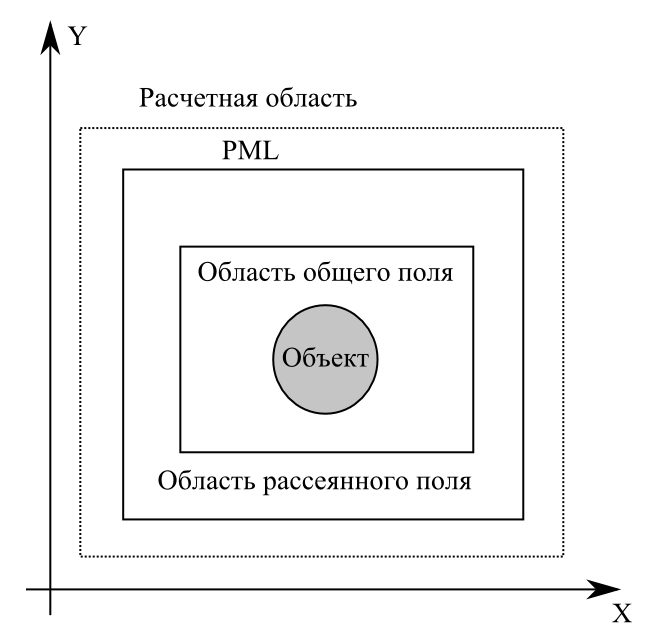
\includegraphics[width=0.5\textwidth]{graphics/tfsf-subdivision-example}
\caption{Пример разбиения расчетной области.}
\label{fig:Tfsf:SubdivisionExample}
\end{figure}
